\RequirePackage{silence}
\WarningFilter{titlesec}{Non standard sectioning command}
\WarningFilter{scrreprt}{Usage of package}
\WarningFilter{scrreprt}{Activating an ugly workaround}

% **************************************************
% Document Class Definition
% **************************************************
\documentclass[%
	paper=A4,					% paper size --> A4 is default in Germany
	twoside=true,				% onesite or twoside printing
	openright,					% doublepage cleaning ends up right side
	parskip=full,				% spacing value / method for paragraphs
	chapterprefix=true,			% prefix for chapter marks
	11pt,						% font size
	headings=normal,			% size of headings
	bibliography=totoc,			% include bib in toc
	listof=totoc,				% include listof entries in toc
	titlepage=on,				% own page for each title page
	captions=tableabove,		% display table captions above the float env
	draft=false,				% value for draft version
]{scrreprt}%

% **************************************************
% Debug LaTeX Information
% **************************************************
%\listfiles

% **************************************************
% Information and Commands for Reuse
% **************************************************
\newcommand{\thesisTitle}{Bright Galaxies as Redshift Tracers for Dark Siren Cosmology}
\newcommand{\thesisName}{Muhammad Khuzaifa Naveed}
\newcommand{\thesisSubject}{Master Thesis}
\newcommand{\thesisDate}{AY 2024-2025}
\newcommand{\thesisDateSubmission}{June, 2025}
\newcommand{\thesisVersion}{First Draft}

%\newcommand{\thesisFirstReviewer}{Jane Doe}
%\newcommand{\thesisFirstReviewerUniversity}{\protect{Ghent University}}
%\newcommand{\thesisFirstReviewerDepartment}{Department of Clean Thesis %Style}
%
%\newcommand{\thesisSecondReviewer}{John Doe}
%\newcommand{\thesisSecondReviewerUniversity}{\protect{Ghent University}}
%\newcommand{\thesisSecondReviewerDepartment}{Department of Clean Thesis Style}

\newcommand{\thesisFirstSupervisor}{Prof. Dr. Archisman Ghosh}
\newcommand{\thesisSecondSupervisor}{Cezary Turski}

\newcommand{\thesisUniversity}{\protect{Ghent University}}
\newcommand{\thesisUniversityDepartment}{Department of Physics and Astronomy}
%\newcommand{\thesisUniversityInstitute}{Institut for Clean Thesis Dev}
\newcommand{\thesisUniversityGroup}{Ghent Gravity Group}
\newcommand{\thesisUniversityCity}{Ghent}
\newcommand{\thesisUniversityStreetAddress}{Proeftuinstraat 86}
\newcommand{\thesisUniversityPostalCode}{9000}

% **************************************************
% Load and Configure Packages
% **************************************************
\usepackage{pdfpages}
\usepackage{subcaption}
\usepackage{svg}
\usepackage[printonlyused,withpage]{acronym}
\usepackage{hyperref}
\usepackage{tocloft}
\usepackage[toc,acronym]{glossaries}
\usepackage[utf8]{inputenc}		% defines file's character encoding
\usepackage[english]{babel} % babel system, adjust the language of the content
\usepackage[					% clean thesis style
	figuresep=colon,%
	sansserif=false,%
	hangfigurecaption=false,%
	hangsection=true,%
	hangsubsection=true,%
	colorize=full,%
	colortheme=bluemagenta,%
% LLT: Use biber if using UTF8 encoding
 	bibsys=bibtex,%
%	bibsys=biber,%
	bibfile=bib-refs,%
	bibstyle=authoryear,%
]{cleanthesis}

\hypersetup{					% setup the hyperref-package options
	pdftitle={\thesisTitle},	% 	- title (PDF meta)
	pdfsubject={\thesisSubject},% 	- subject (PDF meta)
	pdfauthor={\thesisName},	% 	- author (PDF meta)
	plainpages=false,			% 	-
	colorlinks=true,			% 	- colorize links?
	pdfborder={0 0 0},			% 	-
	breaklinks=true,			% 	- allow line break inside links
	bookmarksnumbered=true,		%
	bookmarksopen=true,			%
        linkcolor= black,
        anchorcolor = ctcoloraccessory,
        citecolor = ctcoloraccessory,
        filecolor = ctcoloraccessory,
        menucolor = red,
        runcolor = ctcoloraccessory,
        urlcolor = ctcoloraccessory
}

\renewcommand{\cftloftitlefont}{\thesischapterfont\huge\bfseries}
\renewcommand{\cftfigfont}{\helv\normalsize}

\renewcommand{\cftlottitlefont}{\thesischapterfont\huge\bfseries}
\renewcommand{\cfttabfont}{\helv\normalsize}

\renewcommand{\cfttoctitlefont}{\thesischapterfont\huge\bfseries}
\renewcommand{\cftchapfont}{\thesisparagraphfont\normalsize\bfseries}
\renewcommand{\cftsecfont}{\helv}
\renewcommand{\cftsubsecfont}{\helv}
% **************************************************
% Document CONTENT
% **************************************************
\begin{document}

% --------------------------
% rename document parts
% --------------------------
%\renewcaptionname{ngerman}{\figurename}{Abb.}
%\renewcaptionname{ngerman}{\tablename}{Tab.}
\renewcaptionname{english}{\figurename}{Fig.}
\renewcaptionname{english}{\tablename}{Tab.}

% --------------------------
% Front matter
% --------------------------
\pagenumbering{roman}			% roman page numbing (invisible for empty page style)
\pagestyle{empty}				% no header or footers
% !TEX root = ../thesis-example.tex
%
% ------------------------------------  --> cover title page
\includepdf[pages=-]{cover.pdf}

% ------------------------------------  --> main title page
\begin{titlepage}
	\pdfbookmark[0]{Titlepage}{Titlepage}
	\tgherosfont

	%{\Large \thesisUniversity} \\[4mm]
	\includegraphics[width=3cm]{gfx/logo_ugent_en.png} \\[2mm]
	\textsf{\thesisUniversityDepartment} \\
	%\textsf{\thesisUniversityInstitute} \\
	\textsf{\thesisUniversityGroup} \\

	\vfill
	%{\large \thesisSubject} \\[5mm]
	{\LARGE \color{ctcolortitle}\textbf{\thesisTitle} \\[10mm]}
	{\large \thesisName} \\

	\vfill
	%\begin{minipage}[t]{.27\textwidth}
	%	\raggedleft
	%	\textit{1. Reviewer}
	%\end{minipage}
	%\hspace*{15pt}
	%\begin{minipage}[t]{.65\textwidth}
	%	{\Large \thesisFirstReviewer} \\
	%  	{\small \thesisFirstReviewerDepartment} \\[-1mm]
	%	{\small \thesisFirstReviewerUniversity}
	%\end{minipage} \\[5mm]
	%\begin{minipage}[t]{.27\textwidth}
	%	\raggedleft
	%	\textit{2. Reviewer}
	%\end{minipage}
	%\hspace*{15pt}
	%\begin{minipage}[t]{.65\textwidth}
	%	{\Large \thesisSecondReviewer} \\
	%  	{\small \thesisSecondReviewerDepartment} \\[-1mm]
	%	{\small \thesisSecondReviewerUniversity}
	%\end{minipage} \\[10mm]
	\begin{minipage}[t]{.27\textwidth}
		\raggedleft
		\textit{Promotor} \\
		\textit{Day-to-day supervisor}
	\end{minipage}
	\hspace*{15pt}
	\begin{minipage}[t]{.65\textwidth}
		\thesisFirstSupervisor\\
		\thesisSecondSupervisor
	\end{minipage} \\[10mm]

	\thesisDate \\

\end{titlepage}


% ------------------------------------  --> lower title back for single page layout
\hfill
\vfill
{
	\small
	\textbf{\thesisName} \\
	\textit{\thesisTitle} \\
	\thesisSubject, \thesisDate \\
	%Reviewers: \thesisFirstReviewer\ and \thesisSecondReviewer \\
	Promotor: \thesisFirstSupervisor \\
	Day-to-day supervisor: \thesisSecondSupervisor \\[1.5em]
	\textbf{\thesisUniversity} \\
	\textit{\thesisUniversityGroup} \\
	%\thesisUniversityInstitute \\
	\thesisUniversityDepartment \\
	\thesisUniversityStreetAddress \\
	\thesisUniversityPostalCode\, \thesisUniversityCity
}
		% INCLUDE: all titlepages
\cleardoublepage

% !TEX root = ../thesis-example.tex
%
%************************************************
% Declaration
%************************************************
\pdfbookmark[0]{Declaration}{Declaration}
\chapter*{Declaration}
\label{sec:declaration}
\thispagestyle{empty}

I hereby declare that this thesis is the result of my own work and has not been submitted for any degree or qualification at any other academic institution. All sources of information used have been appropriately acknowledged and referenced.

I affirm that the research, analysis, and implementation described in this thesis were carried out independently. To improve the clarity, grammar, and structure of the text, large language models (such as ChatGPT and Gemini) were used for language refinement. In addition, generative AI was employed to assist in generating code for one specific figure, limited to its visual representation. These tools were not used for scientific interpretation or data analysis.

All intellectual contributions, scientific reasoning, and conclusions presented in this work are entirely my own.

\bigskip

\noindent\textit{\thesisUniversityCity, \thesisDateSubmission}

\smallskip

\begin{flushright}
	\begin{minipage}{5cm}
		\rule{\textwidth}{1pt}
		\centering\thesisName
	\end{minipage}
\end{flushright}

%*****************************************
%*****************************************

\clearpage
\newpage
\mbox{}

% !TEX root = ../thesis-example.tex
%
\pdfbookmark[0]{Acknowledgement}{Acknowledgement}
\chapter*{Acknowledgement}
\label{sec:acknowledgement}
\vspace*{-10mm}
%First and foremost, I would like to express my sincere gratitude to my promotor, Prof. Dr. Archisman Ghosh, for his guidance, support, and insightful feedback throughout this project. I am especially thankful for his flexibility and willingness to accommodate my schedule, which enabled me to work effectively under my own constraints. I am particularly grateful to my day-to-day supervisor, Cezary Turski, whose mentorship, patience, and consistent encouragement were instrumental throughout every phase of this thesis. His feedback, technical guidance, and responsiveness were key in helping me navigate both conceptual challenges and practical implementation. I deeply appreciate the time and effort they invested in my progress, and their understanding in adjusting to my working rhythm.
%
%I am also thankful to the GWCats collaboration for providing a valuable forum of expertise and exchange that informed several aspects of this research. A special thanks goes to Prof. Marcelle Soares-Santos for her early advice and for introducing me to the \texttt{BUZZARD} mock catalog, which shaped an important part of this thesis.
%
%I gratefully acknowledge the use of computational resources provided by the LIGO Laboratory computing clusters, which enabled the analysis performed in this work. Special appreciation is due to the developers and maintainers of the \texttt{gwcosmo} pipeline, the \texttt{GWSim} package, and the galaxy catalogs used in this work, including \texttt{GLADE+} and \texttt{BUZZARD}, whose open resources made this research possible.
%
%On a personal note, I am deeply grateful to my family for their unwavering support. In particular, I would like to thank my parents, whose love, encouragement, and sacrifices have made all of this possible. I am especially thankful to my mother, whose genuine interest in my work, despite having no background in the field, has always meant a great deal to me. Their belief in me has been the foundation of my academic journey, and I dedicate this work to them with immense gratitude. I also like to thank my friends for their timely distractions and unwavering companionship, which served as crucial reminders that there is, in fact, life beyond academic jargon and late-night analyses.
%
%Finally, I would like to thank everyone who contributed, directly or indirectly, to the successful completion of this thesis. Your support has meant more than words can convey.
%
\vspace{2em}
\noindent Muhammad Khuzaifa Naveed
 % INCLUDE: acknowledgement
\cleardoublepage

\pagestyle{plain}				% display just page numbers
% !TEX root = ../thesis-example.tex
%
\pdfbookmark[0]{Abstract}{Abstract}
\chapter*{Abstract}
\label{sec:abstract}
\vspace*{-13mm}
Gravitational-wave (GW) observations have introduced a powerful, independent method to measure the Hubble constant, $H_0$, through the use of so-called \textit{standard sirens}. This thesis investigates the use of \textit{dark sirens}, GW events without electromagnetic counterparts, for cosmological inference. In particular, it explores whether selecting the brightest galaxies as redshift tracers can improve the redshift prior and enhance the precision of $H_0$ estimation. By focusing on the most luminous galaxies, we partially mitigate the effects of catalog incompleteness currently plaguing dark siren measurements, effectively extending the reach of the catalog for cosmological analysis. Using the \texttt{gwcosmo} inference pipeline and the \texttt{GLADE+} galaxy catalog, a series of brightness-ranked percentiles were tested on a subset of the GWTC-3 catalog. The results show that moderate pruning improves $H_0$ constraints, while aggressive cuts lead to information loss and potential bias. Simulated mock data challenges using the \texttt{BUZZARD} catalog support this approach and reveal a lower pruning threshold near 30\% of the brightest galaxies. This method enhances the utility of incomplete galaxy catalogs in dark siren cosmology and contributes to the broader effort to resolve the Hubble tension.\\
\\

{\usekomafont{chapter} Samenvatting}\label{sec:abstract-nl}\\

\vspace*{-2mm}
Zwaartekrachtgolven (GW) bieden een krachtig en onafhankelijk middel om de Hubbleconstante, $H_0$, te meten via de zogenaamde \textit{standaard-sirenes}. Deze scriptie onderzoekt het gebruik van \textit{donkere sirenes}, GW-waarnemingen zonder elektromagnetische tegenhangers, voor kosmologische inferentie. In het bijzonder wordt nagegaan of het selecteren van de helderste sterrenstelsels als roodverschuivingstracers de $z$-prior kan verbeteren en zo de precisie van de $H_0$-schatting kan verhogen. Door ons te richten op de lichtkrachtigste sterrenstelsels wordt de impact van de onvolledigheid van bestaande sterrenstelscatalogi, een bekende uitdaging bij analyses met donkere sirenes, gedeeltelijk gemitigeerd, waardoor de effectieve diepte van de catalogus toeneemt. Met behulp van de \texttt{gwcosmo}-pipeline en de \texttt{GLADE+}-catalogus werd een reeks helderheidspercentielen getest op een subset van de GWTC-3-catalogus. De resultaten tonen aan dat gematigde afkappingen leiden tot een scherpere $H_0$ schatting, terwijl agressieve afkappingen resulteren in informatiederving en mogelijke bias. Gesimuleerde Mock Data Challenges met de \texttt{BUZZARD}-catalogus ondersteunen deze aanpak en wijzen op een praktische ondergrens van ongeveer 30\% van de helderste sterrenstelsels. Deze methode vergroot de toepasbaarheid van onvolledige sterrenstelscatalogi in donkere sirene-kosmologie en levert een bijdrage aan de bredere inspanningen om de Hubble-spanning op te lossen.
		% INCLUDE: the abstracts
\cleardoublepage

\setcounter{tocdepth}{2}		% define depth of toc
\tableofcontents				% display table of contents
\cleardoublepage

\phantomsection
\addcontentsline{toc}{chapter}{\listfigurename}
\label{lof:toc}

\listoffigures
\cleardoublepage

\phantomsection
\addcontentsline{toc}{chapter}{\listtablename}
\label{lot:toc}

\listoftables
\cleardoublepage

\phantomsection
\addcontentsline{toc}{chapter}{List of Abbreviations}
{\setkomafont{chapter}{\thesischapterfont\huge\bfseries} % Match the chapter font
\chapter*{List of Abbreviations}}
\begin{acronym}[ABC]\itemsep8.0pt
  \acro{GW}{Graviational-Wave}
  \acro{CBC}{compact binary coalescence}
  \acro{LVK}{LIGO, Virgo, KAGRA}
  \acro{BNS}{binary neutron star}
  \acro{BBH}{binary black hole}
  \acro{NSBH}{neutron star black hole}
  \acro{EM}{Electromagnetic}
  \acro{LOS}{line-of-sight}
  \acro{SNR}{signal-to-noise ratio}
  \acro{SNe}{supernovae}
  \acro{GWTC}{Gravitational-Wave Transient Catalog}
  \acro{BCG}{Brightest Cluster Galaxy}
  \acro{MDC}{Mock Data Challenge}
  \acro{DES}{Dark Energy Survey}
  \acro{KDE}{kernel density estimation}
  \acro{CMB}{cosmic microwave background}
  \acro{SH0ES}{Supernovae H0 for the Equation of State}
  \acro{HST}{Hubble Space Telescope}
  \acro{SNe Ia}{Type Ia supernovae}
  \acro{TRGB}{Tip of the Red Giant Branch}
  \acro{BAO}{Baryon Acoustic Oscillations}
  \acro{JWST}{James Webb Space Telescope}
\end{acronym}

\cleardoublepage

% --------------------------
% Body matter
% --------------------------
\pagenumbering{arabic}			% arabic page numbering
\setcounter{page}{1}			% set page counter
\pagestyle{maincontentstyle} 	% fancy header and footer

\chapter{Introduction}
\label{chap:introdustion}

\section{The Hubble Tension}
\begin{itemize}
    \item Explain traditional methods of measuring $H_0$ (e.g. SNe, CMB, BAO)
    \item Discuss the discrepancy between local measurements (e.g. SNe) and CMB measurements
    \item Introduce the concept of the Hubble tension and its significance in cosmology
\end{itemize}

\section{Standard Siren Cosmology}
\begin{itemize}
    \item Explain the concept of standard sirens and their role in cosmology
    \item Discuss the use of gravitational waves (GWs) as standard sirens
    \item Introduce the idea of using electromagnetic (EM) counterparts to improve distance measurements
    \item Discuss the advantages and limitations of standard sirens compared to traditional methods
    \item Shorter expalantion compared to chapter 2
\end{itemize}

\section{Thesis Objectives}
\begin{itemize}
    \item Explain the core idea of the thesis: using brightness-ranked galaxy catalogs to improve the precision of $H_0$ measurements
    \item Discuss the motivation behind using brightness-ranked catalogs
    \item BUZZARD
\end{itemize}

\chapter{Gravitational-Wave Cosmology}
\label{chap:dark-siren-cosmology}

\section{Standard Siren Cosmology}

The detection of \ac{GW} from \acp{CBC} have opened a transformative avenue in modern cosmology. These events acts as \textit{standard sirens}, the gravitational analog of standard candles, as the luminosity distance ($d_L$) to a \ac{GW} source is directly encoded in the strain amplitude and frequency evolution of the \ac{GW}. The amplitude, corrected for antenna pattern and inclination, provides a direct, calibration-free distance measurement under the assumption of general relativity.

From~\citet{maggiore2007gravitational}, the strain measured by a GW detector can be expressed as:
\begin{align}
h(t) = \frac{4}{d_L} \left( \frac{G\mathcal{M}_z}{c^2} \right)^{5/3}
       \left( \pi f(t) \right)^{2/3} F(\iota, \psi, \theta, \phi)
\label{eq:gw_strain}
\end{align}
where:
\vspace{-1em}
\begin{itemize}
    \item $h(t)$ is the strain measured at time $t$,
    \vspace{-1em}
    \item $d_L$ is the luminosity distance to the source,
    \vspace{-1em}
    \item $\mathcal{M}_z = (1+z)\mathcal{M}$ is the redshifted chirp mass,
    \vspace{-1em}
    \item $f(t)$ is the instantaneous GW frequency,
    \vspace{-1em}
    \item $F(\iota, \psi, \theta, \phi)$ is a function that captures the detector response depending on inclination angle $\iota$, polarization angle $\psi$, and sky position $(\theta, \phi)$.
\end{itemize}

The amplitude scaling with $1/d_L$ makes it possible to extract the luminosity distance directly from the signal, once the source's intrinsic properties and orientation are marginalized over. Furthermore, the $1/d_L$ scaling, in comaprison to the $1/d_L^2$ scaling of \ac{EM} signals, means that \ac{GW} signals allow observations of sources at much larger distances, making them ideal for cosmological applications.

The direct self-calibrated measurement of the luminosity distance from the \ac{GW} signal is a key advantage of standard sirens over traditional \ac{EM} standard candles. This is in stark contrast to traditional \ac{EM} standard candles, such as \ac{SNe}, where the distance is inferred from the observed flux and requires a calibration step to account for the intrinsic brightness of the source.The \ac{GW} signal is also less affected by the intergalactic medium, as it is not subject to scattering or absorption like \ac{EM} signals. This allows for a more direct measurement of the distance to the source not affected by dust extinction or other astrophysical uncertainties that plague \ac{EM} observations. This makes \ac{GW} standard sirens a powerful tool for cosmology.

The concept of standard sirens was first introduced by Bernard F. Schutz, who noted that if the redshift of a \ac{GW} source can be measured, one could use \ac{GW} events to trace the  expansion history of the universe, in particular an independent measurement of the Hubble constant ($H_0$) \citep{schutz1986determining}. This is due to the realtion bewteen the luminosity distance, redshift and the Hubble constant, in a flat \(\Lambda\)CDM cosmology, being:
\begin{align}
    d_L = \frac{c(1+z)}{H_0} \int_0^z \frac{dz'}{\sqrt{(1+z')^3\Omega_m + \Omega_\Lambda}}
\end{align}

Unlike traditional \ac{EM} methods, which require cross-calibration across multiple rungs of the distance ladder (parallax, Cepheids, SNe Ia) with each step introducing uncertainties that compound, the standard siren approach provides a direct cosmological probe. This reduces systematic uncertainties and provides an independent check on other $H_0$ measurement techniques, possibly providing a solution to the Hubble tension, the current discrepancy between local and global measurements of the Hubble constant \citep{Riess:2019cxk,Planck:2018vyg}.

However, a key limitation is that while \ac{GW} detectors provide a precise measurement of $d_L$, they do not directly measure the redshift. This necessitates an independent redshift measurement to place the source on the Hubble diagram. For \textit{bright sirens}, this redshift is obtained from the host galaxy identified via the electromagnetic counterpart. In contrast, for \textit{dark sirens}, the redshift is inferred statistically by cross-referencing the \ac{GW} localization volume with galaxy catalogs or by leveraging population-based methods, as discussed in the following sections.

This forms the basis for \textit{standard siren cosmology}, where \ac{GW} sources are used as cosmic rulers. Over the past decade, this idea has transitioned from theoretical speculation to experimental reality, primarily through observations made by the \ac{LVK} collaboration. The first \ac{GW} event, \textbf{GW150914}, was detected in 2015, marking the beginning of a new era in astrophysics and cosmology \citep{abbott2016gw150914}. Since then, the \ac{LVK} collaboration has detected numerous \ac{GW} events, including binary black hole mergers, binary neutron star mergers, and neutron star-black hole mergers. These observations have provided valuable insights into the nature of gravity, the formation of compact objects, and the expansion history of the universe.

\section{Bright vs. Dark Sirens}
Standard sirens fall into two broad categories: \textit{bright sirens} and \textit{dark sirens}, depending on whether an electromagnetic counterpart is detected.

Bright sirens are rare but powerful. A prime example is \textbf{GW170817}, a \ac{BNS} merger detected by LIGO-Virgo in 2017, which was accompanied by a short gamma-ray burst and subsequent kilonova \citep{LIGOScientific:2017adf}. This multi-messenger event enabled the unambiguous identification of its \textit{host galaxy, NGC 4993}, providing both distance (from \ac{GW}) and redshift (from optical spectroscopy) measurements. The resulting Hubble constant measurement was a major milestone demonstrating that \ac{GW} observations could offer an independent and competitive cosmological probe \citep{LIGOScientific:2017adf}.

Such bright sirens provide a straightforward route to cosmological inference, using independent distance and redshift measurements. However, bright sirens require specific astrophysical conditions: the emission of \ac{EM} signals strong enough to be detected, accurate sky localization, and timely follow-up by optical telescopes. Such conditions are only met for a small fraction of \ac{CBC} events, especially those involving neutron stars. Majority of the observed mergers, especially \acp{BBH} do not produce detectable \ac{EM} counterparts, and are thus classified as dark sirens.

In the absence of a direct redshift measurement, dark sirens require a \textit{statistical approach}. This involves cross-matching the sky localization and distance posterior from the \ac{GW} event with a galaxy catalog covering the relevant region. The redshift information of a number of candidate galaxies is then used to statistically infer the likely redshift distribution of the source. This is done by constructing a \textit{\ac{LOS} redshift prior} for each \ac{GW} event, which is then used to infer the Hubble constant. The LOS redshift prior is constructed by taking into account the galaxy number density and redshift distribution within the localization volume of the \ac{GW} event. The \ac{GW} localization volume is typically much larger than the volume of a galaxy, leading to a large number of galaxies that could potentially host the \ac{GW} event. This results in a large number of potential redshift measurements, which can be used to construct a more accurate \ac{LOS} redshift prior.

The statistical nature of dark sirens allows for the inclusion of a larger number of events, as it does not rely on the detection of an \ac{EM} counterpart. This is particularly important for \ac{BBH} events, which are more common and have a higher detection rate than \ac{BNS} events. 
%The \ac{LVK} collaboration has detected a large number of \ac{BBH} events, many of which are dark sirens. 
The \ac{LVK} collaboration has detected numerous dark siren events, which have been used to constrain the Hubble constant and test cosmological models.

As the number of \ac{BBH} detections increases with each observing run, dark sirens will dominate the future of standard siren cosmology. However, this statistical method introduces new complexities and depends heavily on the quality and completeness of the galaxy catalog used, which plays a pivotal role in the reliability of the inferred Hubble constant. The incompleteness of the galaxy catalog can lead to biases in the inferred redshift distribution, which can affect the accuracy of the Hubble constant measurement. This is particularly important for dark sirens, as they rely on the statistical association of \ac{GW} events with galaxies in the catalog. State of the art dark siren methods have been developed to mitigate these issues, but they still rely on the quality and completeness of the galaxy catalog used. The next section discusses the current state of the art in dark siren cosmology, including the challenges and limitations of existing methods.

\section{State of the Art Dark Siren Methods}
The statistical framework for dark siren cosmology has evolved rapidly. Early implementations relied on basic overlap between GW localization volumes and precompiled galaxy catalogs. The first generation of tools, including \texttt{gwcosmo}~\citep{gray2020cosmological, gray2022pixelated, gray2023joint} and \texttt{icarogw}~\citep{mastrogiovanni2021importance, mastrogiovanni2024icarogw}, introduced a more rigorous Bayesian framework: for each \ac{GW} event, a \textit{\ac{LOS} redshift prior} is constructed using galaxy number counts and redshifts, weighted by host probability, typically modeled using stellar mass proxies such as $K$-band luminosity.

One major challenge in this process is that current galaxy catalogs, such as \textbf{GLADE+} \citep{dalya2022glade+}, are incomplete beyond low redshift (typically $ z > 0.2 - 0.3$). This incompleteness leads to a nontrivial \textit{out-of-catalog} term in the redshift prior, which must be modeled analytically using a \textit{Schechter luminosity function}. This function estimates the number density of missing faint galaxies, often assuming fixed parameters (e.g., $M_*,\alpha$) calibrated from deep surveys. If this modeling is inaccurate, the resulting posterior for $H_0$ can be biased or artificially broadened.

Despite these challenges, dark siren methods have been successfully applied to increasingly large datasets. The \ac{LVK} collaboration has published joint analyses using \ac{CBC} events from the \textbf{O1, O2,} and \textbf{O3} observing runs. For instance,~\cite{abbott2021gravitational, abbott2023constraints} presented cumulative constraints on $H_0$ using numerous \ac{CBC} events, demonstrating convergence toward a 10--15\% precision regime, albeit still limited by catalog systematics.

These analyses highlight the potential of dark sirens to provide competitive cosmological constraints, especially as galaxy catalogs improve and detection rates increase. Future observing runs, such as O4 and O5, are expected to significantly enhance the statistical power of dark siren cosmology, potentially reducing uncertainties in $H_0$, providng better constraints on cosmological model, and testing the validity of general relativity on cosmological scales. The next generation of \ac{GW} detectors, such as the \textbf{Einstein Telescope} and \textbf{Cosmic Explorer}, will further enhance the sensitivity and detection rates of \ac{GW} events, opening up new avenues for cosmological exploration.

\subsection{Redshift Inference Methods}
In dark siren cosmology, two principal strategies exist for inferring the redshift of gravitational-wave sources: the \textit{catalog-based method}(\textbf{CITATION NEEDED}) and the \textit{population-based method}~\citep{ezquiaga2022spectral}. The catalog method, discussed earlier, statistically associates GW sources with galaxies from a survey by constructing a redshift prior along each line of sight, derived from galaxy positions and redshifts within the GW localization volume. This approach captures the clustering of galaxies and allows for redshift inference when direct \ac{EM} counterparts are absent, but suffers from incompleteness at higher redshifts and spatial variation in survey depth(\textbf{CITATION NEEDED}). Conversely, the population method, often referred to as the \textit{spectral siren approach}, leverages features in the observed distribution of source-frame binary parameters, especially masses, which are redshifted in the detector frame. If the intrinsic mass distribution contains recognizable structure (e.g., a cutoff or peak), its displacement due to cosmic redshift can break the mass-redshift degeneracy, enabling cosmological inference independent of galaxy surveys~\citep{ezquiaga2022spectral}. However, this approach is sensitive to modeling assumptions about the underlying binary population. 

Recent work has sought to improve robustness by combining dark siren methods with \textit{spectral sirens}, extracting redshift information from the observed mass distribution of \ac{GW} sources under population synthesis assumptions~\citep{ezquiaga2022spectral}. These hybrid approaches aim to reduce dependence on incomplete catalogs and mitigate selection biases while extracting maximal cosmological information from current GW detections. Recently, both \texttt{gwcosmo} and \texttt{icarogw} have been updated to support such joint inference schemes~\citep{gray2023joint, mastrogiovanni2024icarogw}.

%Although powerful and refined, these methods are still limited by the incompleteness of the currently available galaxy catalog. This thesis aims to tackle this incompleteness problem, by refining the construction of the redshift prior. This is done by \textit{restricting the galaxy catalog to its brightest subset}, effectively making the catalog more complete. The rationale being that bright galaxies are better cataloged and more reliably associated with massive halos, which are more likely to host detectable GW events. By selectively using only the top $XX\%$ of galaxies by $K$-band luminosity, one can reduce the \textit{out-of-catalog contribution}, thereby increasing precision without strongly biasing the result. The upcoming chapters describe and validate this approach using real and mock data.

\subsection{Galaxy Weighting Choices}
In the construction of the \ac{LOS} redshift prior, each host galaxy is weighted by the probability of hosting a \ac{GW} event. This probability is typically modeled as a function of the galaxy's luminosity, and relies on the assumption that the merger host probability of a galaxy is related to its luminosity in a specific band. The choice of band remains uncertain, with different bands correlating with different aspects. The blue band, for instance, correlates with star formation rate and is therefore appropriate for mergers with short time delays (coalescence shortly after formation), while the near-infrared band correlates with the total luminous mass and is thus appropriate for mergers with longer time delays (mergers in older, more evolved galaxies). It is not known how exactly galaxy color is correlated with the merger rate.

For modelling the out-of-catalog contribution, a Schechter luminosity function is assumed, which describes the distribution of galaxy luminosities in a given band. Wrong assumptions on the Schechter parameters, or incorrect description of selection biases can lead to biases in the inferred Hubble constant. The key assumption in constructing the out-of-catalog contribution is that the galaxy catalog is magnitude limited, i.e. galaxies are not detected only because they are too faint. If other selection biases (based on e.g., colors or spectral features) were present, the out-of-catalog contribution would be biased, leading to an incorrect estimate of the redshift prior \citep{abbott2023constraints}. 

If the assumption of a magnitude-limited catalog is valid, then the luminosity function of the galaxy catalog would match the assumed Schechter function at its bright end, and then start to decrease as it reaches the corresponding absolute magnitude threshold. As can be seen in Figure~\ref{fig:luminosity_function}, this is indeed the case for the $K$-band luminosity function, which is well described by the assumed Schechter function. The $B_J$-band luminosity function, on the other hand, is not well described by the assumed luminosity function, and the assumption of a magnitude-limited catalog is not valid as there seem to be some additional missing galaxies at low redshift. This could lead to an incorrect estimate of the out-of-catalog contribution, and therefore an incorrect estimate of the redshift prior \citep{abbott2023constraints}.

\begin{figure}[h!]
    \centering
    \includegraphics[width=\textwidth]{figures/apjac74bbf15_hr.jpg}
    \caption[The $B_J$-band luminosity function and the $K$-band luminosity function for the \texttt{GLADE+} catalog.]{The $B_J$-band luminosity function (left) and the $K$-band luminosity function (right) for the \texttt{GLADE+} catalog. The solid lines show the luminosity function of the catalog, while the dashed lines shows the assumed Schechter function. The vertical dashed line indicates the median absolute magnitude threshold for galaxy detection. The bright end of the $K$-band luminosity seems to match the assumed Schechter function, while the $B_J$-band luminosity function does not. This indicates that the assumption of a magnitude-limited catalog is not valid for the $B_J$-band luminosity function \citep{abbott2023constraints}.}
    \label{fig:luminosity_function}
\end{figure}

For this reason, traditionally, the $K$-band luminosity has been used for galaxy weighting in \ac{GW} cosmology inference pipelines. This is also due to the fact that the $K$-band luminosity is better correlated with the stellar mass of the galaxy, making it a more reliable tracer of the underlying matter distribution \citep{strazzullo2006near,sureshkumar2021galaxy,abbott2023constraints}. 

However, this choice is not without its limitations. The $K$-band luminosity is not always available for all galaxies in the catalog, leading to potential biases in the selection of galaxies used to construct the redshift prior. For example, the $K$-band luminosity is only aialable for about 1 million galaxies in the \texttt{GLADE+} catalog, which is a small fraction of the total number of galaxies in the catalog. This can lead to uncertainties in the redshift prior, which can in turn affect the inferred value of the Hubble constant. However, this affect should be relatively small, as we are interested in the overall matter distribution, and the $K$-band luminosity is a good tracer of the underlying matter distribution. This also forms the basis for this thesis, as we will be using the brightest galaxies in the $K$-band to trace the underlying matter distribution for improved $H_0$ inference as discussed in the next section.

\section{Refining the Redshift Prior: Brightest Galaxies as Tracers}
The current state of the art in dark siren cosmology relies heavily on the quality and completeness of the galaxy catalog used to construct the \ac{LOS} redshift prior. 
%The incompleteness of the galaxy catalog can lead to significant uncertainties in the redshift prior, which can in turn affect the inferred value of the Hubble constant. This is particularly important for dark sirens, as they rely on the statistical association of \ac{GW} events with galaxies in the catalog. 
The incompleteness of the galaxy catalog can lead to biases in the inferred redshift distribution, which can affect the accuracy of the Hubble constant measurement. State of the art dark siren methods have been developed to mitigate these issues, but they still rely on the quality and completeness of the galaxy catalog used.

%While the statistical dark siren framework is powerful, its precision is ultimately limited by catalog incompleteness and the resulting need to model out-of-catalog galaxies. 
One strategy to mitigate this limitation is by refining the construction of the redshift prior by focusing on the \textit{brightest galaxies}, which are more likely to be catalogued and potentially better tracers of the underlying matter distribution. This would effectively make the catalog more complete and increase precision without introducing significant bias. The rationale is that the brightest galaxies are more likely to be associated with massive halos, which are more likely to host detectable \ac{GW} events. The brightest galaxies are also more likely to be catalogued, as they are easier to detect and measure. These galaxies would also crudely trace the underlying matter distribution, as they are more likely to be associated with massive halos. This would be particulary useful for dark sirens, as they rely on the statistical association of \ac{GW} events with galaxies in the catalog. By replacing the redshift of the true host galaxy with the redshift of a nearby bright galaxy in the catalog, the small error incurred would be insignificant compared to the overall uncertainty in the redshift prior and the luminosity distance measurement.

This approach is similar to the \textit{\ac{BCG}} method used in traditional cosmology, where the brightest galaxy in a cluster is used as a standard candle. The \ac{BCG} method has been shown to be effective in reducing the scatter in distance measurements and improving the precision of cosmological constraints \citep{lauer2014brightest}. By applying a similar approach to dark sirens, one can potentially improve the precision of the inferred Hubble constant without introducing significant bias.

To implement this approach, we define a subset of the galaxy catalog, \texttt{GLADEPXX}, which includes only the top $XX\%$ of galaxies ranked by $K$-band luminosity, as the $K$-band luminosity is better associated with the mass of the galaxies \citep{strazzullo2006near,sureshkumar2021galaxy}. The construction of the LOS redshift prior is then modified to account for this restricted catalog. Specifically, the Schechter luminosity function is adjusted to reflect the brighter subset, making the out-of-catalog contribution smaller, effectively mmaking the catalog more complete.

This modified prior is then used in the Bayesian framework to infer the Hubble constant. The next chapter provides a detailed description of the methodology, including the selection criteria for \texttt{GLADEPXX}, the modeling of the out-of-catalog part and the validation of this approach using mock data.

\textbf{TODO:} Make a figure visualizing the idea!
\chapter{Data}
\label{chap:data}


The foundation of any standard siren cosmological analysis lies in the quality, completeness, and coverage of the data. In this thesis, we rely on two primary data sources: \ac{GW} observations from the \acf{LVK} detectors, and galaxy catalogs providing \ac{EM} redshift information. These datasets are used in tandem to statistically contruct a redshift prior for each \ac{GW} event and ultimately to constrain the Hubble constant $H_0$.

\section{\ac{GW} Event Data}

\subsection{The GWTC-3 Catalog}

The \ac{GW} data used in this study are obtained from the \textit{\acf{GWTC}}~\citep{abbott201gwtc1, abbott2021gwtc2, abbott2023gwtc3, abbott2024gwtc21}. This catalog comprises all \ac{CBC} events detected during the three observing runs (O1, O2, and O3) of the Advanced LIGO and Virgo detectors. \ac{GWTC} includes over 93 confident detections, primarily \acf{BBH} mergers, along with a few \acf{NSBH} and \acf{BNS} systems.

For each event, the catalog provides posterior samples for key source parameters inferred through Bayesian parameter estimation. These include the detector-frame component masses $(m_{1}^{\text{det}}, m_{2}^{\text{det}})$, the luminosity distance $d_L$, sky location (right ascension $\alpha$ and declination $\delta$), orbital inclination angle $\iota$, chirp mass $\mathcal{M}$, and various spin parameters (e.g., $\chi_{\text{eff}}$, $\chi_1$, $\chi_2$). These samples form the basis for constructing the luminosity distance posterior and are essential inputs to the standard siren inference pipeline.

%\subsection{Evant Parameter Estimation?}
%Is it needed to mention the parameter estimation? I think not.
%
\subsection{Event Selection Criteria}

To focus our analysis on dark siren cosmology, we restrict our sample to events that do not have any confirmed electromagnetic counterpart (i.e., no associated kilonova or GRB), have a network \ac{SNR} exceeding 11, have somewhat good sky localization, and are accompanied by publicly available posterior samples for distance and sky position.

These criteria are designed to ensure both the statistical robustness of the inference and compatibility with existing galaxy catalogs. After applying these cuts, a subset of 47 events, with 42 \acp{BBH}, 3
\acp{NSBH}, and 2 \acp{BNS}, is retained for cosmological analysis.

\subsection{Distance Posteriors and Sky Localization}

Each event is characterized by a posterior distribution over the three-dimensional localization volume, typically encoded using the HEALPix format. The posterior provides the probability density $p(d_L, \alpha, \delta)$, where $d_L$ is the luminosity distance and $(\alpha, \delta)$ denote right ascension and declination.

These distance posteriors are crucial for constructing the \ac{LOS} redshift prior when cross-matched with galaxy catalogs. Events with poor localization or multimodal distance distributions contribute more uncertainty to the inferred $H_0$, emphasizing the importance of event quality.

\subsection{Assumptions About the Source Population}
\label{sec:source_population}

Although this thesis primarily focuses on statistical redshift modeling, it is important to acknowledge that the cosmological inference also depends on assumptions about the source population. For instance, \texttt{gwcosmo} allows one to specify priors on:
\begin{itemize}
  \item Merger rate evolution with redshift, typically modeled as \( R(z) \propto (1+z)^\kappa \)
  \vspace{-1em}
  \item Mass distributions of the binaries
\end{itemize}

For our analysis we assume that \acp{CBC} follow a Madau-Dickinson merger redshift evolution model \citep{madau2014cosmic}:
\begin{align}
    R(z) = R_0(1+z)^{\gamma}\frac{1+(1+z_p)^{-(\gamma+\kappa)}}{1+\left( \frac{1+z}{1+z_p}\right)^{\gamma + \kappa}}
\end{align}
Here $R_0$ is the local merger rate, $\kappa$ the high-z slope, $\gamma$ the low-z slop and $z_p$ the break-point. All the assumed priors, taken from \citet{abbott2023gwtc}, are given in Table \ref{tab:Madau}.

To model the source population, for \ac{BBH}, we use power-law with a Gaussian peak mass model, with powerlaw slope $\alpha$, the mean of the Gaussian $\sigma_g$, the width of the peak $\mu_g$, and the relative weight between power-law and the peak $\lambda_g$. We also assume the minimum and maximum masses for the black hole distribution. For neutron stars we assume that mass is uniformly distributed between $M_{\mathrm{min, NS}}$ and $M_{\mathrm{max, NS}}$. All the assumed priors, taken from \citet{abbott2023gwtc}, are given in Table \ref{tab:mass_dist}.

\begin{table}[h!]
    \small
    \centering
    \caption{Priors on merger rate shape parameters.}
    \label{tab:Madau}
    \begin{tabular}{c l}
        \hline
        \textbf{Parameter} & \textbf{Prior} \\
        \hline
         $R_0$ & $1/R_0$ (implicit) \\
         $\kappa$ & $2.86$ \\
         $\gamma$ & $4.59$ \\
         $z_p$ & $2.47$ \\
         \hline
    \end{tabular}
\end{table}

\begin{table}[h!]
    \small
    \centering
    \caption{Priors on the mass model parameters.}
    \label{tab:mass_dist}
    \begin{tabular}{c l}
        \hline
        \textbf{Parameter} & \textbf{Prior} \\
        \hline
         $\alpha$ & $3.78$ \\
         $\sigma_g$ & $3.88$ \\
         $\mu_g$ & $32.27$ \\
         $\lambda_g$ & $0.03$ \\
         $M_{min,\mathrm{BH}}$ & $4.98M_{\odot}$ \\
         $M_{max,\mathrm{BH}}$ & $112.5M_{\odot}$ \\
         $M_{min,\mathrm{NS}}$ & $1.0M_{\odot}$ \\
         $M_{max,\mathrm{NS}}$ & $3.0M_{\odot}$ \\
         \hline
    \end{tabular}
\end{table}

\newpage

\section{\ac{EM} Galaxy Catalogs}

\subsection{The \texttt{GLADE+} Galaxy Catalog}

For redshift information, we use the \texttt{GLADE+} galaxy catalog~\citep{dalya2022glade+}, an extended version of the original \texttt{GLADE} catalog~\citep{dalya2018glade}, designed for \ac{GW} follow-up. \texttt{GLADE+} is a composite catalog that combines several large surveys to achieve all-sky coverage:
\vspace{-1em}
\begin{itemize}
  \item 2MASS XSC and 2MPZ: infrared-based all-sky surveys~\citep{skrutskie2006two, bilicki2013two} 
  \vspace{-1em}
  \item WISExSCOS: photometric redshifts from the \ac{WISE} and the SuperCOSMOS survey~\citep{bilicki2016wise}
  \vspace{-1em}
  \item HyperLEDA: spectroscopic redshift survey~\citep{makarov2014hyperleda}
  \vspace{-1em}
  \item SDSS DR16Q: quasar catalog~\citep{lyke2020sloan}
\end{itemize}

As of the latest release, \texttt{GLADE+} includes over 22 million objects with available positions, redshifts (spectroscopic or photometric), and photometry in multiple bands, most critically the $K$-band~\citep{dalya2022glade+}.

\subsection{Catalog Completeness}
\label{sec:luminosity_function}

A significant limitation of \texttt{GLADE+} is its incompleteness beyond redshift $z \sim 0.3$. While the catalog is approximately complete for bright galaxies at low redshift, its coverage of fainter galaxies or more distant regions is limited. This incompleteness introduces a bias when performing statistical redshift inference, as missing galaxies contribute to the out-of-catalog part of the redshift prior.

To address this, the \texttt{gwcosmo} pipeline models the galaxy population, for the out-of-catalog region, using a truncated Schechter luminosity function~\citep{schechter1976analytic} in the $K$-band. The Schechter function describes the distribution of galaxy luminosities and is given by:
\begin{align}
    \phi(M) \propto 10^{0.4(\alpha + 1)(M - M^*)} \exp[-10^{0.4(M - M^*)}]
\end{align}
where \( M \) is the absolute magnitude in the $K$-band, $M^*$ is the characteristic magnitude, and $\alpha$ is the faint-end slope. For our analysis, we adopt the standard parameters: $\alpha = -1.09$, $M^*_{K} = -23.39 + 5\log h$, consistent with \citet{kochanek2001k}, and truncate at $M^*_{K,\mathrm{min}} = -27.00 + 5\log h$ and $M^*_{K,\mathrm{max}} = -19.00 + 5\log h$.

\subsection{Redshift Uncertainty Modeling}

Redshift measurements in \texttt{GLADE+} are heterogeneous. Spectroscopic redshifts are generally precise, but photometric redshifts can have uncertainties on the order of $\sigma_z \sim 0.01-0.05$. These uncertainties are modeled by convolving the redshift of each galaxy with a Gaussian of fixed width, an assumption used in constructing the redshift prior.

Additionally, to reduce systematic error, galaxies with unphysical redshifts or unreliable photometry are filtered out during preprocessing. The net result is a cleaned, sky-localized, and redshift-tagged galaxy distribution that can be used for \ac{LOS} prior construction.

Furthermore, $K$-corrections are applied in \texttt{gwcosmo} following \citet{kochanek2001k}, and the apparent magnitude thresholds $m_{\mathrm{thr}}$ are computed per HEALPix pixel as a median apparent magnitude in a given pixel, giving a $K$-band threshold of 13.5 on average.

\subsection{$K$-band Luminosity as Host Probability Proxy}

In dark siren analysis, we must assign each galaxy a probability of being the true host. Following common practice, this probability is assumed to scale with stellar mass, for which $K$-band luminosity serves as a good proxy~\citep{strazzullo2006near,sureshkumar2021galaxy}. The host probability  $p_i$ for each galaxy is given by:
\begin{align}
    p_i \propto L_{K, i}
\end{align}
This choice is motivated by the assumption that more massive galaxies are more likely to host \acp{CBC} events. While simplistic, it provides a reasonable baseline.
\chapter{GLADE+ Bright Galaxies as Redshift Tracers}
\label{chap:methodology}

%The core idea investigated in this thesis is the use of \textbf{bright galaxies} as redshift tracers for \ac{GW} events. The \texttt{GLADE+} galaxy catalog is a comprehensive database of galaxies in the local Universe, but it suffers from incompleteness at high redshifts. This incompleteness arises from the limited depth of the catalog, which is primarily designed to cover the local Universe, owing to the sensitivity constraints of the current \ac{EM} telescope. We overcome this limitation by focusing on the brightest galaxies in the catalog, which are more likely to be well-represented and can provide a more accurate estimate of the redshift of \ac{GW} events. This essentiaally makes the catalog deeper and more complete at high redshifts, while allowing us to use the \texttt{GLADE+} catalog as a proxy for the underlying matter distribution in the Universe.
The core idea investigated in this thesis is the use of \textbf{bright galaxies} as redshift tracers for \ac{GW} events. The \texttt{GLADE+} galaxy catalog is a comprehensive compilation of galaxies in the local Universe, designed primarily to support multi-messenger follow-up observations. However, it suffers from incompleteness at higher redshifts due to the limited sensitivity of current \ac{EM} surveys.

To mitigate this limitation, we focus on the brightest galaxies in the catalog, which are more likely to be detected at higher redshifts and better trace the large-scale structure. By applying a brightness-based pruning strategy, we effectively enhance the redshift reach and completeness of the catalog, allowing \texttt{GLADE+} to serve as a more accurate proxy for the underlying matter distribution relevant to dark siren cosmology.

The results and methodology developed in this thesis have been submitted for peer review to the \textit{\ac{MNRAS}} and are available as a preprint on \texttt{arXiv}~\citep{naveed2025dark}, contributing to the growing body of research in \ac{GW} cosmology.

\section{Bright Galaxy Subsets}
The analysis begins with the construction of \textbf{bright galaxy subsets}, denoted \texttt{GLADEPXX}, where only the top $XX\%$ of galaxies by cumulative $K$-band luminosity are included. The $K$-band luminosity is chosen as it is better associated with the mass of the galaxies \citep{strazzullo2006near,sureshkumar2021galaxy}. Limiting the analysis to these bright subsets allows us to:
\vspace{-1em}
\begin{itemize}
  \item Reduce the out-of-catalog correction by focusing on bright galaxies likely to be well-represented.
  \vspace{-1em}
  \item Improve the signal-to-noise ratio of the statistical redshift prior.
  \vspace{-1em}
  \item Minimize the inclusion of poorly characterized or faint galaxies.
\end{itemize}

The bright galaxy subsets are defined by selecting galaxies based on their absolute magnitude, which is inferred from their redshift and apparent magnitude. For a given subset, the dimmest galaxy sets the absolute magnitude limit, $M_{\mathrm{max}}$, for that subset. This limit is then used in the Schechter luminosity function to adjust the out-of-catalog contribution, effectively reducing its impact. By focusing on the brightest galaxies, we assume that they trace the mass distribution in the Universe more effectively, and are more likely to host \ac{CBC} events.

This approach improves the completeness of the galaxy catalog in the high-redshift regime, as the out-of-catalog contribution becomes smaller. Figure~\ref{fig:z_dist} illustrates how the redshift distribution shift towards higher values making the catalog more complete, highlighting the effectiveness of this method in probing deeper $z$--ranges.

\begin{figure}[h!]
  \centering
  \includegraphics[width=0.7\linewidth]{figures/z_dist_perc.png}
  \caption[Normalized redshift distributions $p(z)$ for the \texttt{GLADE+} galaxy catalogue and its brightest percentiles.]{Normalized redshift distributions $p(z)$ for the full \texttt{GLADE+} galaxy catalogue (blue) and the brightest percentiles (other curves). Each subset, labeled \texttt{GLADEPXX}, includes only the top XX\% brightest galaxies in the $K$-band. Focusing on increasingly brighter subsets shifts and sharpens the redshift distribution, effectively probing deeper ranges in $z$.}
  \label{fig:z_dist}
\end{figure}

\subsection{Trade-Offs and Limitations}

While bright subsets reduce catalog incompleteness, they may inadvertently exclude genuine host galaxies, especially if those lie in less luminous systems or in underrepresented regions of the catalog. The effectiveness of these cuts depends on the intrinsic distribution of host galaxies, the depth and completeness of the original catalog, and the accuracy of $K$-band photometry. 
%The effectiveness of these cuts therefore depends on:
%\vspace{-1em}
%\begin{itemize}
%  \item The depth and completeness of the original catalog.
%  \vspace{-1em}
%  \item The intrinsic distribution of host galaxies.
%  \vspace{-1em}
%  \item The accuracy of $K$-band photometry.
%\end{itemize}

One major limitation of this approach is that brightest galaxies may not be representative of the overall galaxy population, as they may be biased towards certain types of galaxies or regions of the sky. This effect is however mitigated by the fact that we are using the $K$-band luminosities, which are good tracer for the stellar mass \citep{strazzullo2006near,sureshkumar2021galaxy}, and in turn the overall matter distribution. Furthermore, the bright galaxy subsets are constructed from the \texttt{GLADE+} catalog, which is designed to be a complete and representative sample of galaxies in the local Universe. This means that the bright galaxy subsets are likely to be representative of the overall galaxy population, and give a crude estimate of the matter distribution, even if they are not a complete sample.

Estimating the true redshift of a \ac{GW} event by the nearest brightest galaxies is supposed to have a negligible effect on the results. This is because the bright galaxies are more likely to be located in regions of high density, such as galaxy clusters or groups, which are also likely to host \ac{GW} events. This means that the bright galaxies are likely to be located in the same large-scale structure as the \ac{GW} event, and thus provide a good estimate of the redshift of the event. 

One important thing to note is that while the use of a bright subset enhances the completeness of the catalogue at high redshifts, it also introduces a trade-off. If the brightness cut is too restrictive, the exclusion of galaxies may lead to a loss of information and in turn an underrepresentation of the overall matter distribution, potentially biasing the results. One needs to carefully balance these considerations by comparing different brightness thresholds. A moderate brightness cut will maximize the benefit in terms of depth without incurring significant bias. The appropriate brightness cut can be established only via a set of astrophysics-motivated large-scale simulations. A \ac{GW} \textit{\ac{MDC}}, detailed in the next chapter, using the simulated \texttt{BUZZARD} galaxy catalog from the \ac{DES} Collaboration~\citep{DES:2019jmj,DES:2021bwg}.  
%It is designed to determine the optimal brightness threshold which maximizes the measurement precision with bright subsets while keeping the biases in control. Tests performed in the process will help refine the methodology and ensure that the improved constraints on the Hubble constant are robust against additional systematic uncertainties.

Another thing to note is that due to to the brightness cut, we may lose the low-redshift galaxies, in turn losing information in the nearby Universe. This can be easily overcome in the future by combining the use a complete galaxy catalog in the nearby Universe, with the bright galaxy subsets in the high-redshift regime. This will allow us to have a complete galaxy catalog in the nearby Universe, while still being able to probe deeper redshifts using the bright galaxy subsets. But this is not a trivial task, as it would require a smooth transition between the two cases. But nonetheless, this is a good first step towards improving the completeness of the galaxy catalog and future work could further refine this approach by using different redshift tracers in different redshift regimes, such as using the bright galaxy subsets in the high-redshift regime, and a complete galaxy catalog in the nearby Universe.

While the bright galaxy subsets may not be a perfect representation of the overall galaxy population, they are still a useful tool for improving the completeness of the galaxy catalog and reducing the out-of-catalog correction. The error incurred by using the bright galaxies as redshift tracers may be small compared to the current errors in luminosity distance measurements from the \ac{GW} events, this may become a problem in the future as the \ac{GW} measurements become more precise. In this case, one may need to use more sophisticated methods to estimate the redshift of the \ac{GW} event, such as more complex models of the galaxy population, but for now this is a good first step towards improving the completeness of the galaxy catalog and reducing the out-of-catalog correction, by leveraging the currently available \ac{EM} data.

%In Chapters~\ref{chap:results} and~\ref{chap:mockdata}, we quantify these trade-offs using both real data and mock catalogs.

\begin{figure}[h!]
  \centering
  \begin{subfigure}{0.32\textwidth}
    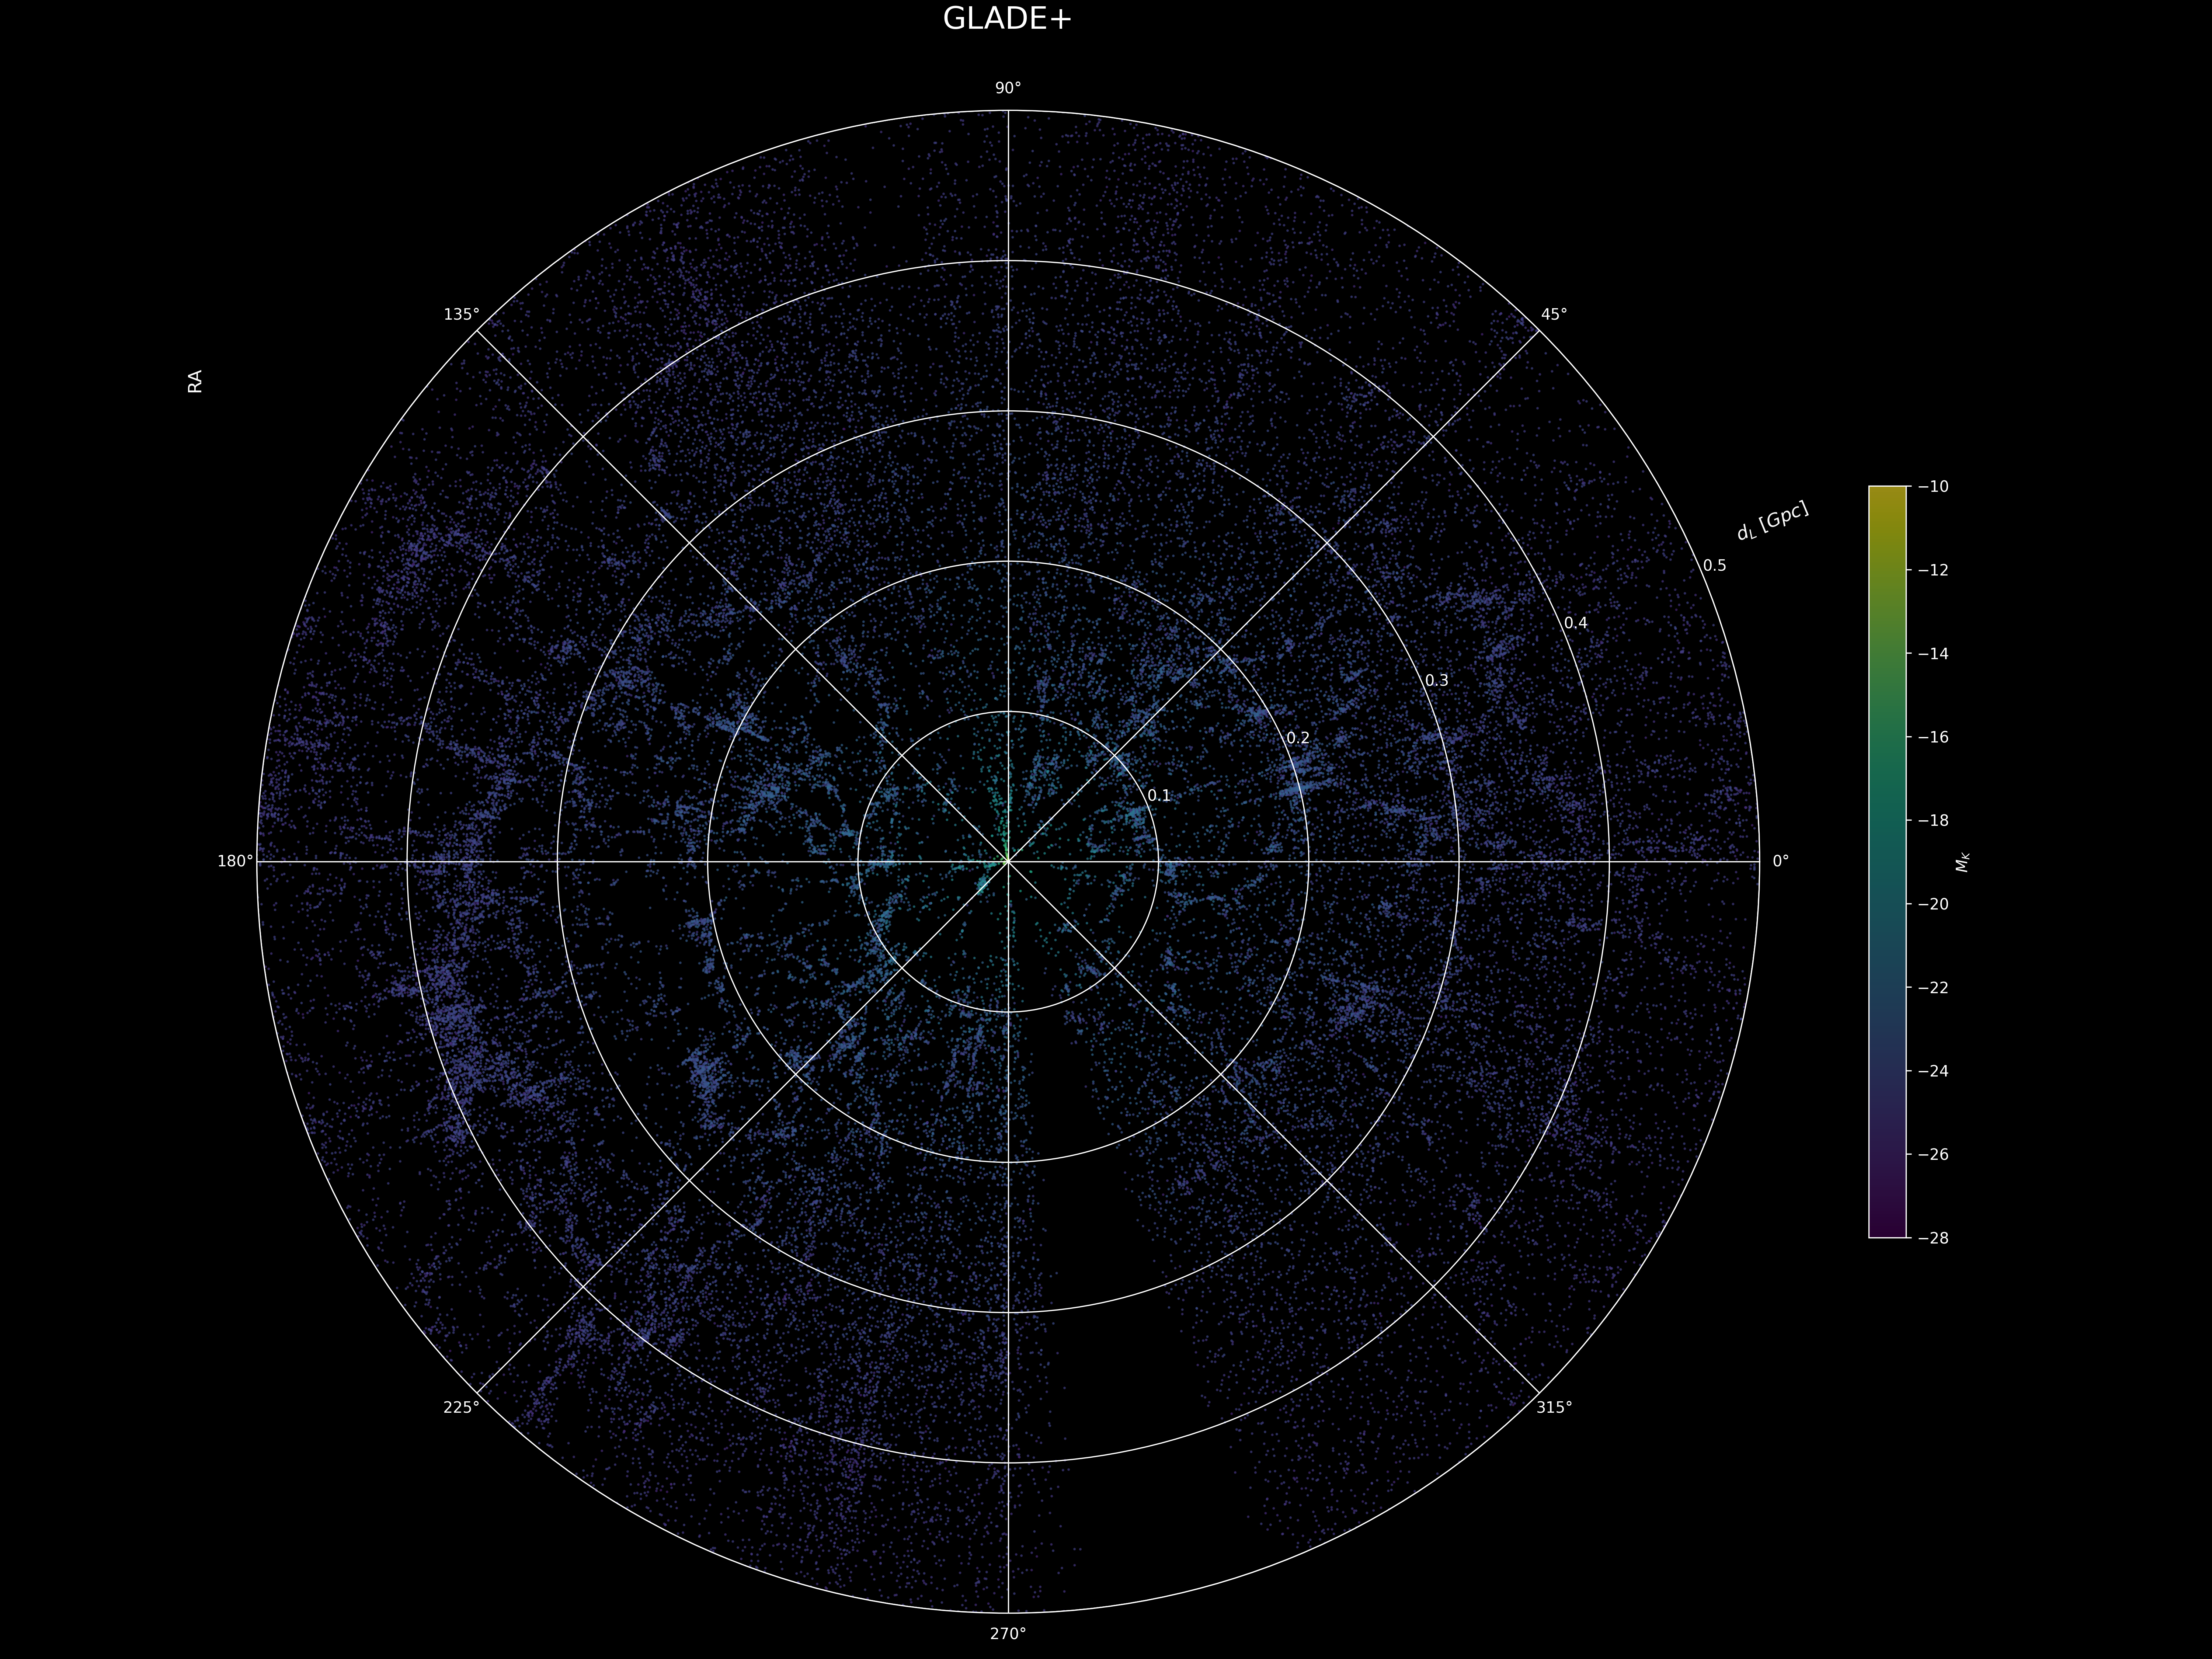
\includegraphics[width=\linewidth]{figures/test_frame_g_0.png}
    \label{fig:gladep100}
  \end{subfigure}
  \begin{subfigure}{0.32\textwidth}
    \includegraphics[width=\linewidth]{figures/test_frame_g_1.png}
    \label{fig:gladep90}
  \end{subfigure}
  \begin{subfigure}{0.32\textwidth}
    \includegraphics[width=\linewidth]{figures/test_frame_g_2.png}
    \label{fig:gladep80}
  \end{subfigure}
  \vspace{0.5em}
  \begin{subfigure}{0.32\textwidth}
    \includegraphics[width=\linewidth]{figures/test_frame_g_3.png}
    \label{fig:gladep70}
  \end{subfigure}
  \begin{subfigure}{0.32\textwidth}
    \includegraphics[width=\linewidth]{figures/test_frame_g_4.png}
    \label{fig:gladep60}
  \end{subfigure}
  \begin{subfigure}{0.32\textwidth}
    \includegraphics[width=\linewidth]{figures/test_frame_g_5.png}
    \label{fig:gladep50}
  \end{subfigure}
  \vspace{0.5em}
  \begin{subfigure}{0.32\textwidth}
    \includegraphics[width=\linewidth]{figures/test_frame_g_6.png}
    \label{fig:gladep40}
  \end{subfigure}
  \begin{subfigure}{0.32\textwidth}
    \includegraphics[width=\linewidth]{figures/test_frame_g_7.png}
    \label{fig:gladep30}
  \end{subfigure}
  \begin{subfigure}{0.32\textwidth}
    \includegraphics[width=\linewidth]{figures/test_frame_g_8.png}
    \label{fig:gladep20}
  \end{subfigure}

  \vspace{0.5em}

  \begin{subfigure}{0.32\textwidth}
    \includegraphics[width=\linewidth]{figures/test_frame_g_9.png}
    \label{fig:gladep10}
  \end{subfigure}
  \begin{subfigure}{0.64\textwidth}
    \centering
    \includegraphics[width=\linewidth]{figures/test_frame_g_colorbar.png}
    \vspace{0.02em}
  \end{subfigure}

  \caption[Spatial distribution of galaxies from the GLADE+ galaxy catalog and its subsets.]{Spatial distribution of galaxies from the GLADE+ catalog and its bright subsets, employed for dark standard siren cosmology. The plots show a 10-degree slice in declination, centered at $0^\circ$, with the radial coordinate representing luminosity distance $d_L$ (in Gpc) and the angular coordinates being right ascension (RA). This shows how the bright galaxies trace the large-scale structure of the Universe.}
  \label{fig:dist_gladep}
\end{figure}


\newpage

\section{\Ac{LOS} Redshift Prior}
%We base our analysis on the \texttt{gwcosmo} pipeline \citep{gray2020cosmological,gray2022pixelated,gray2023joint}, which relies on a precomputed \ac{LOS} redshift prior, a prior on the \ac{GW} signal's redshift and direction. This \ac{LOS} redshift prior is used in tandem with the luminosity distance posterior from the \ac{GW} signal, to get a measurement for the Hubble constant $H_0$.

As \texttt{gwcosmo} requires a redshift prior for each \ac{GW} event, we construct a \ac{LOS} redshift prior from the \texttt{GLADE+} galaxy catalog. The \texttt{GLADE+} catalog is a comprehensive database of galaxies in the local Universe, which provides information about their positions, redshifts, and luminosities. This catalog is used to construct a redshift prior for each \ac{GW} event, which is used in tandem with the luminosity distance posterior from the \ac{GW} signal, to get a measurement for the Hubble constant $H_0$.

\subsection{\ac{LOS} Redshift Prior Construction}
The \ac{LOS} redshift prior is constructed from the \texttt{GLADE+} galaxy catalog, which contains a wealth of information about the galaxies in the local Universe. The redshift prior is constructed by taking into account the distribution of galaxies along the line of sight to the \ac{GW} event, as well as their luminosity and redshift. This allows us to obtain a more accurate estimate for the redshift of the \ac{GW} signal, which is crucial for cosmological measurements. The prior is constructed by dividing the sky into HEALPix pixels, and computing the redshift distribution of galaxies in each pixel. The redshift prior is then weighted using the luminosity of the potential host galaxies, allowing us to obtain a more accurate estimate for the Hubble constant.

Furthermore, the prior accounts for the incompleteness of the galaxy catalog, using source population models and the magnitude threshold calculated per pixel, which is particularly important for high-redshift events where the number of galaxies is significantly reduced. This allows us to separate the \ac{LOS} redshift prior into an in-catalog and out-of-catalog contribution.

Taking into account, the fact that the host galaxy can be present, or not, inside the catalog, one can write the \ac{LOS} redshift prior as:
\begin{align}
  p(z|\Omega_i, \Lambda, s, I) =& \iint \sum_{g=G,\bar{G}} p(z, M, m,g|\Omega_i, \Lambda, s, I)~dM dm \\
  =&~p(G|\Omega_i, \Lambda, s, I) \iint p(z, M, m|G,\Omega_i, \Lambda, s, I)~dM dm \nonumber \\
  &+ p(\bar{G}|\Omega_i, \Lambda, s, I) \iint p(z, M, m|\bar{G},\Omega_i, \Lambda, s, I)~dM dm
\end{align}

The first term in the equation represents the contribution from galaxies that are present in the catalog, while the second term represents the contribution from galaxies outside the catalog. The two terms are weighted by their respective probabilities of being present or not in the catalog. The terms inside the integral are the priors on the redshift $z$, absolute magnitude $M$, and apparent magnitude of the galaxies $m$, informed by the galaxy catalog, within the sky area covered by pixel $i$. Here the parameters $G/\bar{G}$ give the presence or absence of the galaxy in the catalog, $\Omega_i$ the sky location of the \ac{GW} event, $\Lambda$ the cosmological and population hyperparameters of interest, $s$ the presence of a \ac{GW} source, and $I$ the additional assumptions which are not excplicitly expressed. One also needs to marginalize over the absolute magnitude $M$ and the apparent magnitude $m$ of the galaxy, as these determine, to the leading order, which galaxiess are present in a flux-limited \ac{EM} survey \citep{gray2023joint}.

%\subsubsection{In-Catalog Contribution}
The integral in the in-catalog term can be expressed as the sum over the possible host galaxies in the catalog, weighted by their respective probabilities of being the host galaxy. These galaxies are weighted by their luminosity, which is a function of the absolute magnitude and redshift. The rationale being that the more luminous, and thus heavier galaxies are more likely to host \ac{CBC} events, and therefore contribute more to the \ac{LOS} redshift prior. This reduces the in-catalog part to a wieghted sum over the galaxies in the catalog, where the galaxies are treated as point sources modeled by a Gaussian. This term can thus be expressed as:
\begin{align}
  \iint p(z, M, m|G,\Omega_i, \Lambda, s, I)~dM dm =& \frac{1}{p(s|G,\Omega_i, \Lambda, I)N_{\mathrm{gal}}(\Omega_i)} \nonumber\\ 
  &\times \sum_{k}^{N_{\mathrm{gal}}(\Omega_i)} p(z|\hat{z}_k) p(s|z, M(z, \hat{m}_k, \Lambda), \Lambda, I)
\end{align}
where the term $p(z|\hat{z}_k)$ represents the probability of a galaxy being at redshift $z$, given its observed redshift $\hat{z}_k$. This term is used to weight the contribution from each galaxy in the catalog, based on its observed redshift.

%\subsubsection{Out-of-Catalog Contribution}
The integral in the out-of-catalog term marginalizes over the possible host galaxies not present in the catalog. This term is more complex, as it requires a model for the distribution of galaxies in the Universe, which is not directly available from the catalog. We use a Schechter luminosity function to model the distribution of galaxies in the Universe, which allows us to estimate the contribution from galaxies outside the catalog. The out-of-catalog term can be expressed as:
\begin{align}
  \iint & p(z, M, m|\bar{G},\Omega_i, \Lambda, s, I)~dM dm \nonumber \\
  &= \frac{1}{p(s|\bar{G},\Omega_i, \Lambda, I)p(\bar{G}|\Omega_i, \Lambda, I)} \nonumber \\ 
  &~~~\times \Bigg[\Theta[z_{\mathrm{cut}} -z] \int_{M(z,m_{\mathrm{thr}}(\Omega_i), \Lambda)}^{M_{\mathrm{max}}(H_0)} p(z,M|\Lambda, I) p(s|z,M,\Lambda,I)~dM \nonumber \\
  &\qquad \quad + \Theta[z-z_{\mathrm{cut}}] \int_{M_{\mathrm{min}}(H_0)}^{M_{\mathrm{max}}(H_0)} p(z,M|\Lambda, I) p(s|z,M,\Lambda,I)~dM \Bigg]
\end{align}
Here we also account for the \ac{EM} selection effects of the catalog. Due to the flux limited nature of the galaxy catalog, the probability of a galaxy being present in the catalog depends on the galaxy's apparent magnitude, and whether it is greater or smaller than apparent magnitude threshold of the catalog along the same line of sight, $m_{\mathrm{th}}(\Omega_i)$. The Heaviside function $\Theta$ is used to separate the two cases of the out-of-catalog contribution, depending on whether the redshift $z$ is below or above a certain threshold $z_{\mathrm{cut}}$. This is due to to the exclusion of galaxies with redshift $z$ greater than $z_{\mathrm{cut}}$ from the catalog, which is a result of unreliable redshift or color information at these higher redshifts.

The term $p(s|z,M,\Lambda,I)$ is the weighting factor for the contribution from each galaxy, based on its luminosity and redshift. The galaxies are weighted by their luminosity in the $K$-band, which is a good tracer of the mass of the galaxies \citep{strazzullo2006near,sureshkumar2021galaxy}. Furthermore, the merger host probability is also taken into account, which is a function of the redshift. This is modeled by a Madau-Dickinson merger rate evolution model \citep{madau2014cosmic}, which describes the evolution of the merger rate with redshift, discussed in Section \ref{sec:source_population}. The term $p(s|z,M,\Lambda,I)$, also incorporates the source population models, used to populate the out-of-catalog contribution. These models are also discussed in Section \ref{sec:source_population}.

The term $p(z,M|\Lambda, I)$ represents the luminosity funtion of the galaxies, taken to be the Schechter luminosity function, discussed in Section \ref{sec:luminosity_function}. The integration limits are set by the minimum and maximum absolute magnitudes of the galaxies, $M_{\mathrm{min}}(H_0)$ and $M_{\mathrm{max}}(H_0)$. These are $H_0$-dependent, as the parameters of the Schechter luminosity function are also $H_0$-dependent, but the final distribution remains insensitive to the exact values of $H_0$ \citep{gray2023joint}.

\section{Results}
In this section we present the main outcomes of our analysis: how applying brightness cuts to the \texttt{GLADE+} catalog alters \ac{LOS} redshift prior for individual events, how these modified priors propagate into the inferred posterior on the Hubble constant $H_0$. It should be noted that while \texttt{gwcosmo} is designed to perform joint population and cosmological inference, we focus here on the impact of the brightness cuts on the \ac{LOS} redshift prior and the resulting $H_0$ posterior. For this reason, we do not perform a full joint inference, but rather use \texttt{gwcosmo} for $H_0$ inference, while keeping the population hyperparameters fixed to the values mentioned in Section~\ref{sec:source_population}.

To test the impact of catalog completeness, we apply successive cuts to the galaxy catalog by selecting only the brightest $XX\%$ of galaxies in $K$-band luminosity, forming subsets labeled \texttt{GLADEPXX}. This process shifts the effective redshift upwards, reducing the number of galaxies but improving the catalog's completeness.

\subsection{\ac{LOS} Redshift Prior}
Figure~\ref{fig:los_prior_gw170809} shows the LOS redshift prior for the event \textbf{GW170809} under different catalog cuts. Bright galaxy subsets (e.g., \texttt{GLADEP20}) result in sharper redshift distributions and reduce the weight of the out-of-catalog term. The low-$z$ tail contributed by faint galaxies in the nearby Universe is also suppressed. Notably, these priors maintain consistency in shape, indicating that bright galaxies are reliable tracers of large-scale structure. The application of a brightness cut significantly modifies the \ac{LOS} redshift distribution. Specifically, the bright galaxy subsets yield an amplified redshift prior at higher distances, effectively extending the reach of the catalogue, somewhat mitigating the incompleteness issues that arise at deeper redshifts. This behavior is qualitatively consistent across events.

\begin{figure}[ht]
  \centering
  \includegraphics[width=0.67\textwidth]{figures/GW170809_zprior.png}
  \caption[LOS redshift prior for GW170809 for different brightness-ranked \texttt{GLADE+} subsets]{LOS redshift prior for GW170809 for different brightness-ranked \texttt{GLADE+} subsets. The full \texttt{GLADE+} catalog (solid blue) is compared to the different subsets. Applying a brightness cut amplifies the prior at higher distances, extending the effective reach of the catalog and partially mitigating incompleteness at greater redshifts.}
  \label{fig:los_prior_gw170809}
\end{figure}

\begin{figure}[h!]
  \centering
  \includegraphics[width=0.67\textwidth]{figures/GW170809_H0.png}
  \caption[$H_0$ posterior distributions for GW170809 using different brightness-ranked \texttt{GLADE+} subsets.]{$H_0$ posterior distributions for GW170809 using different brightness-ranked \texttt{GLADE+} subsets. \texttt{GLADEP20} yields the tightest credible interval. \texttt{GLADEP10} suffers from sparse sampling.}
  \label{fig:h0_gw170809}
\end{figure}

\newpage

\subsection{Hubble Constant Posterior}

\begin{figure}[h!]
    \centering
    \includegraphics[width=0.67\textwidth]{figures/percentile_full_dict.png}
    \caption[Cumulative $H_0$ posterior from the selected dark siren events using full \texttt{GLADE+} and the different subsets.]{Cumulative $H_0$ posterior from the selected dark siren events using full \texttt{GLADE+} (blue) and the different subsets (dashed lines). The brightness-weighted catalog yields a tighter constraint without a significant shift.}
    \label{fig:h0_cumulative}
\end{figure}

\begin{table}
    \small
    \centering
    \caption[$H_0$ MAP values with $68\%$ confidence ranges, alongside the maximum magnitude limits for \texttt{GLADE+} and the different subsets.]{Maximum {\em a posteriori} probabilities with $68\%$ confidence ranges of the $H_0$ posterior distributions alongside the maximum magnitude limits for the different percentiles of the \texttt{GLADE+} galaxy catalogue.}
    \begin{tabular}{c c c }
    \hline
        \textbf{Catalogue} & $M_{K,\mathrm{max}}$ & $H_0~[\mathrm{km}~\mathrm{s}^{-1}\mathrm{Mpc}^{-1}]$ \\ \hline
        \\[-0.8em]
        \texttt{GLADE+} & $-19.00$ & $67.87^{+8.97}_{-10.29}$ \\ 
        \\[-0.8em]
        \texttt{GLADEP90} & $-23.07$ & $68.94^{+9.24}_{-7.55}$ \\
        \\[-0.8em]
        \texttt{GLADEP80} & $-23.62$ & $68.93^{+9.25}_{-7.57}$ \\
        \\[-0.8em]
        \texttt{GLADEP70} & $-23.94$ & $68.63^{+8.61}_{-7.42}$ \\
        \\[-0.8em]
        \texttt{GLADEP60} & $-24.19$ & $68.85^{+7.72}_{-6.43}$ \\
        \\[-0.8em]
        \texttt{GLADEP50} & $-24.14$ & $70.05^{+6.12}_{-5.20}$ \\
        \\[-0.8em]
        \texttt{GLADEP40} & $-24.63$ & $69.94^{+7.46}_{-3.88}$ \\
        \\[-0.8em]
        \texttt{GLADEP30} & $-24.87$ & $74.70^{+4.69}_{-6.58}$ \\
        \\[-0.8em]
        \texttt{GLADEP20} & $-25.15$ & $78.28^{+5.53}_{-4.95}$ \\
        \\[-0.8em]
        \texttt{GLADEP10} & $-25.53$ & $63.46^{+6.39}_{-14.37}$ \\ 
        \\[-0.8em]
        \hline
    \end{tabular}
    \label{tab:h0_stats}
\end{table}

Once one has the \ac{LOS} redshift prior, one can use it to compute the posterior distribution of the Hubble constant $H_0$ given the \ac{GW} event data, as the relation between the redhsift $z$, luminosity distance $d_L$ and the Hubble constant $H_0$ is given by:
\begin{align}
  d_L = \frac{c(1+z)}{H_0} \int_0^z \frac{dz'}{\sqrt{(1+z')^3\Omega_m + \Omega_\Lambda}}
\end{align}
for a flat $\Lambda$CDM cosmology. At lower redshifts, this can be simplified to:
\begin{align}
  d_L \approx \frac{cz}{H_0}
\end{align}
Thus the \ac{LOS} redshift prior, $p(z|\Omega_i, \Lambda, s, I)$, and the luminosity distance posterior, $p(d_L,\Omega\mid\mathrm{GW})$, from the \ac{GW} event data can be combined to obtain the posterior distribution of $H_0$, which can then be used to obtain constraints on the value of $H_0$.

Figure~\ref{fig:h0_gw170809} shows the resulting $H_0$ posteriors for GW170809 under various catalog cuts. As the catalog is restricted to brighter galaxies, the $H_0$ posterior becomes increasingly narrow. For example, \texttt{GLADEP20} yields a visibly tighter posterior compared to the full \texttt{GLADE+}, with a shift in the median. However, the most aggressive cut (\texttt{GLADEP10}) introduces broader tails, likely due to insufficient galaxy sampling in the localization volume.

We repeat this procedure for a subset of \ac{CBC} events from \ac{GWTC}-3 that meet our selection criteria. Figure~\ref{fig:h0_cumulative} shows the combined $H_0$ posterior from the selected dark siren events using the full \texttt{GLADE+} catalog and the different subsets. Table~\ref{tab:h0_stats} summarizes the $H_0$ posteriors for all cuts. The uncertainty is minimized around the \texttt{GLADEP20} subset, showing 30-40\% tighter contraints, while median values shift towards a higher value. While these tighter constraints are promising, the shift in median values could indicate a systematic bias introduced by the brightness cuts. This is particularly evident for the most extreme cut (\texttt{GLADEP10}), which yield a significantly lower median $H_0$ value, likely due to under-sampling and loss of information about the large-scale structure. For less extreme cuts, the median values doesn't show a huge shift. This suggests that moderate brightness cuts could improve precision without introducing much systematic bias.

\subsection{Luminosity Retention}
An important consideration when applying brightness-based cuts to galaxy catalogs is understanding how much of the total luminosity is retained as a function of the chosen percentile cut. Figure~\ref{fig:luminosity_fraction} shows the cumulative fraction of total $K$-band luminosity retained when selecting the brightest $X\%$ of galaxies in the \texttt{GLADE+} catalog.

As the figure illustrates, the retained luminosity decreases rapidly when pruning the catalog based on brightness. At first glance, this might suggest that discarding the fainter galaxies results in the loss of a significant portion of cosmologically relevant information. However, this effect is largely driven by the overwhelming number of faint galaxies, each contributing only marginally to the total light output. 

It is also important to note that the selection is made using the brightest percentiles of the catalog itself, rather than a parametric cut based on a fitted Schechter function. This empirical approach includes all galaxies below a certain magnitude threshold, which accentuates the cumulative effect of the numerous low-luminosity galaxies and contributes to the pronounced loss observed in total luminosity.

\begin{figure}[h]
    \centering
    \includegraphics[width=0.7\textwidth]{figures/luminosity_fraction_vs_percentile_GLADE.png}
    \caption[\texttt{GLADE+} luminosity retention.]{Fraction of total $K$-band luminosity as a function of the brightest $X\%$ of galaxies in the catalog. The steep slope near 100\% reflects the contribution of the numerous dim galaxies to the total luminosity budget.\footnotemark}
    \label{fig:luminosity_fraction}
\end{figure}
\footnotetext{This plot was generated using code partially adapted from scripts provided by Cezary Turski.}

The bright galaxies we retain are intrinsically more luminous and are typically associated with massive halos and central locations in galaxy groups or clusters. These bright, high-mass galaxies are more likely to trace the underlying matter distribution, which is essential for our purpose. By focusing on the top percentiles in brightness, we sacrifice luminosity but preserve the most structurally informative objects.

Therefore, while the pruning strategy leads to a steep loss in integrated light (as shown in the figure), this primarily reflects the exclusion of numerous dim galaxies that do not significantly enhance the galaxy density field used to construct the redshift prior. The retained bright galaxies should still provide a robust tracer of large-scale structure, particularly at higher redshifts where catalog completeness begins to decline.

\subsection{Cost-Benefit Trade-Off}
We observe that the precision of the $H_0$ posterior improves as the catalog is pruned to include only the brightest galaxies, up to an optimal point (around \texttt{GLADEP20}). Beyond this point, the constraints begin to degrade, with the posterior broadening and approaching the result obtained with an empty catalog. This degradation arises from under-sampling the galaxy distribution, highlighting a practical limit to brightness-based pruning.

While brightness cuts can enhance statistical precision by removing noisy or weakly informative galaxies, they also risk excluding key structure-tracing galaxies if pushed too far. This trade-off between precision and completeness must be carefully managed, as overly aggressive cuts can introduce bias and weaken the reliability of cosmological inference. The exact location of the optimal cut may depend on the specifics of the GW event, such as its localization volume, and the characteristics of the underlying galaxy catalog.

This balance is best understood within the framework of the \acf{MDC}, which is discussed in the next chapter. The \ac{MDC} allows us to systematically test how different cuts affect the inferred $H_0$, providing a controlled environment to evaluate potential biases and performance.

Our results suggest that targeting the brightest galaxies in a well-characterized catalog can substantially enhance the precision of $H_0$ measurements from dark sirens. This method serves as a complementary approach to other strategies for mitigating catalog incompleteness, such as joint inference with galaxy clustering or population-based redshift estimation.
%\chapter{Results}
\label{chap:results}

In this chapter, we present the main results of our dark siren cosmology analysis using brightness-ranked subsets of the \texttt{GLADE+} galaxy catalog. We evaluate the impact of applying magnitude cuts on the galaxy sample, compare the resulting \ac{LOS} redshift priors, and show how these choices affect the posterior distribution of the Hubble constant $H_0$. We also assess the precision-bias trade-off associated with aggressive catalog cuts.

\section{LOS Redshit Prior}
The first step in our cosmological inference is computing the \ac{LOS} redshift prior $p(z | \Omega, \Lambda, s, I)$ for each \ac{GW} event and sky pixel $\Omega$. This prior combines the redshift distribution of galaxies in the \texttt{GLADE+} catalog with an analytic model for the out-of-catalog population, as described in Chapter~\ref{chap:methodology}.

To test the impact of catalog completeness, we apply successive cuts to the galaxy catalog by selecting only the brightest $XX\%$ of galaxies in $K$-band luminosity, forming subsets labeled \texttt{GLADEPXX}. This process shifts the effective magnitude threshold upward, reducing the number of galaxies but improving the catalog's completeness above the cut.

Figure~\ref{fig:los_prior_gw170809} shows the LOS redshift prior for the event GW170809 under different catalog cuts. Bright galaxy subsets (e.g., \texttt{GLADEP20}) result in sharper redshift distributions and reduce the weight of the out-of-catalog term. Notably, these priors maintain consistency in shape, indicating that bright galaxies are reliable tracers of large-scale structure. The application of a brightness cut significantly modifies the \ac{LOS} redshift distribution. Specifically, the bright galaxy subsets yield an amplified redshift prior at higher distances, effectively extending the reach of the catalogue, somewhat mitigating the incompleteness issues that arise at deeper redshifts.

\begin{figure}[ht]
    \centering
    \includegraphics[width=0.7\textwidth]{figures/GW170809_zprior.png}
    \caption[LOS redshift prior for GW170809 for different brightness-ranked \texttt{GLADE} subsets]{LOS redshift prior for GW170809 for different brightness-ranked \texttt{GLADE} subsets. The full \texttt{GLADE+} catalog (solid blue) is compared to the different subsets. Applying a brightness cut amplifies the prior at higher distances, extending the effective reach of the catalog and partially mitigating incompleteness at greater redshifts.}
    \label{fig:los_prior_gw170809}
\end{figure}

\section{$H_0$ Posterior}

With \ac{LOS} priors in hand, we compute the posterior distribution for the Hubble constant $H_0$ by combining the GW posterior $p(d_L, \Omega | \text{GW})$ with the redshift prior $p(z | \Omega, \Lambda, s, I)$. This is done using the \texttt{gwcosmo} pipeline for each event.

Figure~\ref{fig:h0_gw170809} shows the resulting $H_0$ posteriors for GW170809 under various catalog cuts. As the catalog is restricted to brighter galaxies, the $H_0$ posterior becomes increasingly narrow. For example, GLADEP20 yields a visibly tighter posterior compared to the full GLADE+, with minimal shift in the median. However, the most aggressive cut (GLADEP10) introduces broader tails, likely due to insufficient galaxy sampling in the localization volume.

\begin{figure}[ht]
    \centering
    \includegraphics[width=0.7\textwidth]{figures/GW170809_H0.png}
    \caption[$H_0$ posterior distributions for GW170809 using full and brightness-cut galaxy catalogs.]{$H_0$ posterior distributions for GW170809 using full and brightness-cut galaxy catalogs. \texttt{GLADEP20} yields the tightest credible interval. \texttt{GLADEP10} suffers from sparse sampling.}
    \label{fig:h0_gw170809}
\end{figure}

We repeat this procedure for a subset of \ac{BBH} events from \ac{GWTC} that meet our selection criteria. Figure~\ref{fig:h0_cumulative} shows the combined $H_0$ posterior from the selected dark siren events using the full \texttt{GLADE+} catalog and the different subsets.

Table~\ref{tab:h0_stats} summarizes the $H_0$ posteriors for all cuts. The uncertainty is minimized around the \texttt{GLADEP20} subset, showing 30-40\% tighter contraints, while median values shift towards a higher value. For less extreme cuts, the median values doesn't show a huge shift. This suggests that moderate brightness cuts improve precision without introducing systematic bias.

\begin{figure}[ht]
    \centering
    \includegraphics[width=0.7\textwidth]{figures/percentile_full_dict.png}
    \caption[Cumulative $H_0$ posterior from the slected dark siren events using full \texttt{GLADE+} and the different subsets.]{Cumulative $H_0$ posterior from the slected dark siren events using full \texttt{GLADE+} (blue) and the different subsets (dashed lines). The brightness-weighted catalog yields a tighter constraint without a significant shift.}
    \label{fig:h0_cumulative}
\end{figure}

\begin{table}
    \centering
    \caption[$H_0$ MAP values with $68\%$ confidence ranges, alongside the maximum magnitude limits for \texttt{GLADE+} and the different subsets.]{Maximum {\em a posteriori} probabilities with $68\%$ confidence ranges of the $H_0$ posterior distributions alongside the maximum magnitude limits for the different percentiles of the GLADE+ galaxy catalogue.}
    \begin{tabular}{c c c }
    \hline
        \textbf{Catalogue} & \textbf{$M_{K, max}$} & \textbf{$H_0~[km~s^{-1}Mpc^{-1}]$} \\ \hline
        \texttt{GLADE+} & -19.00 & $67.87^{+8.97}_{-10.29}$ \\
        \texttt{GLADEP90} & -23.07 & $68.94^{+9.24}_{-7.55}$ \\
        \texttt{GLADEP80} & -23.62 & $68.93^{+9.25}_{-7.57}$ \\
        \texttt{GLADEP70} & -23.94 & $68.63^{+8.61}_{-7.42}$ \\
        \texttt{GLADEP60} & -24.19 & $68.85^{+7.72}_{-6.43}$ \\
        \texttt{GLADEP50} & -24.14  & $70.05^{+6.12}_{-5.20}$ \\
        \texttt{GLADEP40} & -24.63 & $69.94^{+7.46}_{-3.88}$ \\
        \texttt{GLADEP30} & -24.87 & $74.70^{+4.69}_{-6.58}$ \\
        \texttt{GLADEP20} & -25.15 & $78.28^{+5.53}_{-4.95}$ \\
        \texttt{GLADEP10} & -25.53 & $63.46^{+6.39}_{-14.37}$ \\ \hline
    \end{tabular}
    \label{tab:h0_stats}
\end{table}

\section{Cost–benefit trade-off}
We observe that precision improves with increasing brightness until an optimum is reached (near \texttt{GLADEP20}). Beyond this point, the posterior widens again due to under-sampling. This defines a practical limit for catalog pruning. In real applications, the exact optimum may depend on event SNR, catalog completeness, and the merger rate model.

Our results suggest that targeting the brightest galaxies in a well-characterized catalog can substantially improve the statistical precision of $H_0$ constraints from dark sirens. This approach complements other efforts to mitigate catalog incompleteness, including joint inference with galaxy clustering and population-informed redshift estimation.
\chapter{Mock Data Challenge}
\label{chap:MDC}

\section{BUZZARD Mock Catalog}

\section{Results}
%\input{content/Discussion}
\chapter{Conclusion}
\label{chap:conclusion}

The emergence of \ac{GW} astronomy has opened a new frontier in observational cosmology. This thesis has explored the potential of using dark sirens, gravitational-wave events without electromagnetic counterparts, for the inference of the Hubble constant, $H_0$. Specifically, we examined whether refining the galaxy catalog used in the redshift prior, by restricting it to its brightest subsets, to trace the large-scale structure, can improve the cosmological constraints from these events.

\section{Summary of Findings}

We implemented a hierarchical Bayesian inference framework using the \texttt{gwcosmo} pipeline, which combines \ac{GW} luminosity distance posteriors with redshift priors constructed from galaxy catalogs. The galaxy redshift prior was derived using the \texttt{GLADE+} catalog and modified by applying brightness cuts to prioritize the most luminous galaxies in the $K$-band. These subsets, denoted \texttt{GLADEPXX}, were hypothesized to trace large-scale structure more efficiently due to their association with massive halos.

The analysis demonstrated that:
\vspace{-1em}
\begin{itemize}
    \item Brightness-ranked catalogs improve the redshift prior, leading to tighter posteriors on $H_0$ by reducing low-likelihood host candidates in the \ac{GW} localization volume.
    \vspace{-1em}
    \item Moderate pruning yields improvement in $H_0$ precision as compared to using the full catalog, without introducing measurable bias. This improvement is attributed to the enhanced clustering signal from retaining mostly central, high-luminosity galaxies.
    \vspace{-1em}
    \item Aggressive pruning (e.g., \texttt{GLADEP10}) results in degraded constraints and larger uncertainties, as the catalog no longer adequately traces the large-scale structure.
    \vspace{-1em}
    \item A lower bound of approximately 30\% of the brightest galaxies emerges as a practical pruning limit, in the best-case scenario where the brightest galaxies are strictly the central-most galaxies. Below this threshold, significant information about the underlying matter distribution is lost, particularly from central galaxies, increasing the risk of cosmological bias.
    \vspace{-1em}
    \item Mock data challenges using the \texttt{BUZZARD} catalog support the robustness of the brightness-based pruning strategy but also emphasize the importance of catalog completeness, redshift depth, and optimal percentile thresholds. The 30\% structural limit appears consistent across lower magnitude cuts, suggesting that future work should avoid overly aggressive pruning or instead develop hybrid approaches combining full and pruned catalogs, depending on the redshift regime.
\end{itemize}

\section{Limitations}

This work, while comprehensive, has several limitations:
\vspace{-1em}
\begin{itemize}
    \item The number of \ac{GW} events with high \ac{SNR} and good localization remains small, limiting the statistical power of our results.
    \vspace{-1em}
    \item Catalog incompleteness, particularly at high redshifts, introduces uncertainties that are only partially mitigated by brightness cuts.
    \vspace{-1em}
    \item Due to time constraints and several technical challenges encountered with the \texttt{BUZZARD} mock catalog, we were unable to perform a full end-to-end bias quantification from pruning dim galaxies. Nevertheless, partial analyses and theoretical considerations support the proposed 30\% threshold as a conservative lower bound.
    \vspace{-1em}
    \item While a complete end-to-end \acf{MDC} framework has been developed, a few components still require minor refinements and consistency checks before full deployment in future analyses.
    %\vspace{-1em}
    %\item The analysis assumes a fixed $\Lambda$CDM cosmology throughout, exploring extended models may reveal different degeneracies or sensitivities in dark siren inference.
\end{itemize}

\section{Outlook and Future Work}

The outlook for dark siren cosmology is highly promising. With the advent of next-generation \ac{GW} detectors such as Cosmic Explorer~\citep{Evans:CE}, Einstein Telescope~\citep{Abac:ET} and LISA~\citep{LISA:2024hlh}, and deeper galaxy surveys like LSST~\citep{ivezic2019lsst} and Euclid~\citep{mellier2024euclid}, both the number of detected events and the completeness of host catalogs are expected to improve significantly.

Future extensions of this work could include:
\vspace{-1em}
\begin{itemize}
    \item Getting a quantitative estimate of the bias introduced by the brightness cuts, with the devised end-to-end \ac{MDC} framework.
    \vspace{-1em}
    \item Testing for potential biases introduced by brightness cuts using larger and more realistic mock datasets.
    \vspace{-1em}
    \item Developing adaptive redshift priors that vary with localization volume depth, combining full catalogs at low redshift with bright subsets at high redshift.
    \vspace{-1em}
    \item Integrating clustering information or cross-correlations with large-scale structure to improve redshift inference~\citep{afroz2024prospect}.
\end{itemize}

Ultimately, the resolution of the Hubble tension will require a convergence of multiple independent probes. As shown in this thesis, dark sirens, when carefully analyzed, offer a robust and independent route to measuring $H_0$. Furthermore, the use of bright galaxies as tracers of large-scale structure provides a promising avenue for improving the precision of cosmological constraints from \ac{GW} observations. This methodology will play a growing role in the era of multi-messenger cosmology.

\cleardoublepage

% --------------------------
% Back matter
% --------------------------

\setstretch{1.1}
\renewcommand{\bibfont}{\normalfont\small}
\setlength{\biblabelsep}{0pt}
\setlength{\bibitemsep}{0.5\baselineskip plus 0.5\baselineskip}
\printbibliography
\cleardoublepage

% **************************************************
% End of Document CONTENT
% **************************************************
\end{document}
